This work builds upon a dataset released as part of the Baidu KDD Cup 2022 wind power forecasting challenge, featuring high-frequency SCADA (Supervisory Control and Data Acquisition) data from 134 wind turbines owned by Longyuan Power Group. Measurements are recorded every 10 minutes over 245 consecutive days, capturing both operational and environmental conditions of each turbine at a given timestamp. The resulting data forms a dense multivariate time series with rich temporal and spatial structure.

Each row in the dataset includes the turbine identifier (\texttt{TurbID}), a day index (\texttt{Day}), and a timestamp (\texttt{Tmstamp}), alongside 13 numerical signals. These include meteorological variables such as wind speed (\texttt{Wspd}), wind direction (\texttt{Wdir}), external and internal temperatures (\texttt{Etmp}, \texttt{Itmp}), as well as machine state indicators like nacelle yaw angle (\texttt{Ndir}), blade pitch angles (\texttt{Pab1}, \texttt{Pab2}, \texttt{Pab3}), reactive power (\texttt{Prtv}), and the primary output variable, active power (\texttt{Patv}). A separate metadata file provides the GPS coordinates of each turbine, enabling spatial analysis if desired.

\begin{figure}[h]
    \centering
    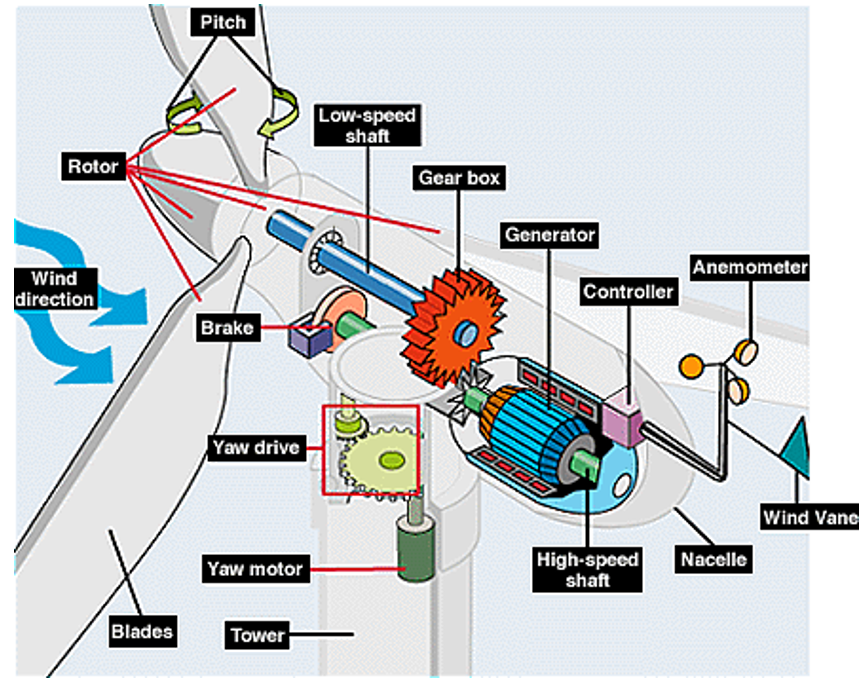
\includegraphics[width=0.7\textwidth]{figures/turbine.png}
    \caption{\url{https://en.wikipedia.org/wiki/File:EERE_illust_large_turbine.gif}}
    \label{fig:turbine}
\end{figure}

To balance complexity with computational feasibility, we restricted our analysis to a representative subset of 10 turbines. This allowed us to maintain the dataset’s temporal and spatial variability while keeping training and evaluation times manageable.


The forecasting task focuses on predicting the short-term future value of \texttt{Patv}. To formalize this as a supervised regression problem, the target was renamed \texttt{patv\_target\_1}, indicating a 10-minute prediction horizon. We also derived several time-based features—such as hour, minute, and day of the week—from each timestamp to help capture cyclical or calendar-related patterns.

To assess generalization over time, we adopted a \textit{temporally stratified cross-validation} strategy. The data was split into eight non-overlapping folds, where each fold consists of 15 consecutive days for training and 7 subsequent days for testing. This simulates deployment scenarios in which models must predict unseen future intervals, accounting for shifts in turbine behavior or weather conditions over time.

Key preprocessing steps were applied before modeling. Missing values in the patv series were filled using forward- and backward-filling, based on the assumption that short-term continuity in power output is a valid approximation. Then, for each turbine, we computed lagged values of \texttt{patv\_target\_1} over a 12-step window (equivalent to two hours of history), allowing models to leverage autoregressive signals. Additionally, lead values were created to define the target outputs in a supervised learning setup.

The resulting dataset consists entirely of numerical features, making it suitable for a variety of learning algorithms, from linear regression to tree ensembles and neural networks. Prior to training, feature scaling was performed using \texttt{StandardScaler} from \texttt{scikit-learn}, fitted only on the training data of each fold and consistently applied to the corresponding test set.

For semi-supervised experiments, we simulated limited-label settings by subsampling 10\%, 20\%, or 70\% of the training data as labeled, while treating the rest as unlabeled. S2RMS leverages these unlabeled examples through iterative pseudo-labeling. CLUS+, on the other hand, handles them natively via symbolic missing targets during model construction. It's important to note that for CLUS experiments, the same fold structure is reused, but without applying external normalization, since the CLUS framework includes its own internal scaling mechanisms. In contrast, supervised baselines like ElasticNet and XGBoost rely on the externally scaled features and are trained only on the labeled subset.

A detailed overview of the dataset structure, including the differences between the original full dataset and the reduced per-fold setting, is provided in Table~\ref{tab:dataset-comparison}.

% \begin{table}[h]
% \centering
% \caption{Dataset summary statistics across folds and supervision levels.}
% \label{tab:dataset-summary}
% \begin{tabularx}{\textwidth}{X r}
% \toprule
% \textbf{Metric} & \textbf{Value} \\
% \midrule
% Lagged Feature Dimensionality & 12 \\
% Total Features (after lag/lead) & 17 \\
% \# Labeled Instances (10\%) & 2,304 \\
% \# Unlabeled Instances (10\%) & 20,736 \\
% \# Labeled Instances (20\%) & 4,608 \\
% \# Unlabeled Instances (20\%) & 18,432 \\
% \# Labeled Instances (70\%) & 16,127 \\
% \# Unlabeled Instances (70\%) & 6,912 \\
% \bottomrule
% \end{tabularx}
% \end{table}

\begin{table}[ht]
\centering
\caption{Comparison between the original dataset and the reduced per-fold version used in experiments.}
\label{tab:dataset-comparison}
\renewcommand{\arraystretch}{1.2}
\begin{tabularx}{\textwidth}{l X X}
\toprule
\textbf{Property} & \textbf{Original Dataset} & \textbf{Per-Fold Dataset} \\
\midrule
Time Span & 245 consecutive days & 22 days (15 for training, 7 for testing) \\
Turbines & 134 & 10 \\
Sampling Frequency & 10 minutes & 10 minutes \\
Total Instances & $\sim$4.7 million & 33,120 per fold \\
Instances per Fold & -- & 23,040 for training \newline 10,080 for testing \\
Labeled Samples (10\%) & -- & $\sim$2,300 \\
Labeled Samples (20\%) & -- & $\sim$4,600 \\
Labeled Samples (70\%) & -- & $\sim$16,000 \\
Unlabeled Samples & -- & 23,040 - Labeled Samples \\
Features & 19 numerical + 1 target & Same \\
Target Variable & PATV & Same \\
\bottomrule
\end{tabularx}
\end{table}
